\documentclass[a4paper,10pt]{article}

\usepackage[utf8]{inputenc}
\usepackage{graphicx}
\usepackage{mathtools}
\usepackage{float}
\usepackage{algorithm2e}
\usepackage{textcomp}
\usepackage{amsfonts}
\usepackage{booktabs}
\usepackage{siunitx}

\newcolumntype{P}[1]{>{\centering\arraybackslash}p{#1}}


\title{SDSS Celestial Objects Classification}
\author{Andrea Sessa \\ \vspace{1cm} \small{Mat. 850082}}
\date{}

\begin{document}

\maketitle

\begin{abstract}
  The project aims to study the problem of dimensionality reduction in the field of astronomy.
  The high number of features involved often makes the job of classifying celestial objects, 
  basing entirely on their spectra, very difficult. The problem of preprocessing high dimensional 
  astronomical data is considered. We refer to the method described in \cite{redshift} to 
  overcome the problem of missing data and the different redshift factor of different object.
  The resulting dataset(which is the starting point for the project) contains information of
  4000 celestial object(such as galaxies, quasars, stars, etc.) each of the samples consists
  of 1000 attributes which describe the electromagnetic radiation over different wavelength(3000 to 8000 angstrom).
  We propose different methodologies to approach the problem of features reduction:
  PCA, ISOMAP, forward features selection and ANOVA F-Test approach;
  The goodness of each method is evaluated over Support Vector Machine(soft margin penalty is tuned by 5-Fold cross-validation)
  considering as metrics accuracy, precision, recall and F1 score.
  Final results shows, in general, how a very small number of features in the can actually capture an high percentage
  of the variance associated with the data and to results identical or better with respect to the case and high number
  of features is used. Moreover final results outline how ISOMAP reveals to be quite ineffective on this particular scenario.
\end{abstract}

\newpage

\tableofcontents

\newpage

\listoffigures

\newpage

\section{Introduction}
  Modern astronomy is concerned with the study of very distant celestial objects ie quasars, galaxies, stars, etc.\newline
  Often this type of classification is performed by analyzing the spectrum emitted by such objects.\newline
  In general the emission spectrum of a chemical element or of a chemical compound is defined as the electromagnetic radiation emitted
  when an atom or a molecule, of the object that we are observing, perform a transition from an high energy states to a low energy state.
  During the decadiment the atom or molecule the electromagnetic is irradiated under the form of photon, the associated photon energy
  (also called flux) is proportional is equal to the energy difference between the two energy states involved in the decadiment.\newline
  The important element is that for a given atom there are many possible electron transition, and each of these transition has a specific
  flux associated.\newline
  The Sloan Digital Sky Survey(henceforth referred as SDSS) is a major imaging and spectroscopic survey using a dedicated 2.5-m wide-angle
  optical telescope at Apache Point Observatory in New Mexico, United States.\newline
  The collection of data started in 2000 and continues up to nowadays(latest data release in June 2013). The dataset comprises almost
  2 millions of spectra coming from different objects.\newline
  Machine learning plays an important role in the task of classifying these objects, given the fact that many times samples include
  more than 1000 features.\newline
  Features in general includes information about the flux associated with a specific wavelength.
  
  \begin{figure}[H]
    \caption{Typical emission spectrum for an emission galaxy}
    \centering
    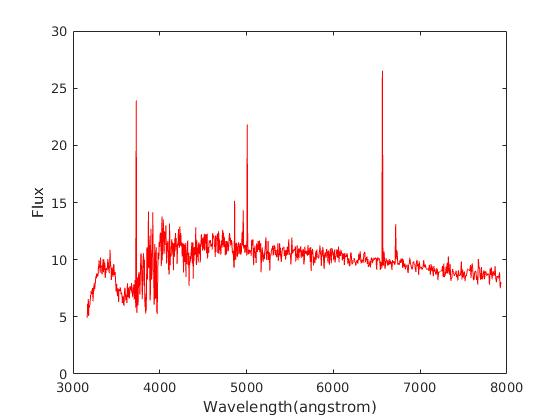
\includegraphics[scale=0.5]{emission_galaxy.jpg}
  \end{figure}
  
  If the input feature vectors have very high dimension, the learning problem can be difficult even if the true function only depends on a small number of those features.
  This is because the many "extra" dimensions can confuse the learning algorithm and cause it to have high variance.
  Hence the problem of features selection become very important in this scenario; this project will try to cast
  some light on the problem by evaluating different approaches over a reduced version of the SDSS dataset.
  
\section{Problem Formulation}
  The overall problem is divided into three main sections:
  \subsection{Features Extraction}
  The first one is the issue of features selection, what follows is a possible formal formulation of the problem:\newline
  The goal is, starting from a number of features $ M = 1000 $, find $M' \ll M$ such that 
  the selected $M'$ features gives the smallest expected generalization error. In more formal terms:\newline\newline
  
  \textit{Given a set of functions $y = f(x,\alpha)$ we want to find a preprocessing over the data, $\textbf{x} \mapsto (\textbf{x} * \sigma)$}
  \begin{equation}
    \tau(\sigma, \alpha) = \int \mathrm V(y,f((x*\sigma),\alpha) \,\mathrm{d}p(\textbf{x},y)
  \end{equation}
  \textit{subject to $||\sigma||_0 = M'$,  where $p(x,y)$ is unknown, $x * \sigma = (x_1 \sigma_1, ... , x_M \sigma_M)$ denotes an
  element wise product, $V (.,.)$ is a generic loss function} \newline
  The literature divided the feautures selected methods into two main group
  \begin{itemize}
   \item \textbf{Filter methods} rely on general characteristics of the data to evaluate and to select the feature subsets without
	 involving the chosen learning algorithm. Scores are assigned to each features according to some metrics.\newline
	 A widely-used filter method is to apply a classical univariate ANOVA F-Test. 

   \item \textbf{Wrapper methods} evaluate subsets of features which allows, unlike filter approaches, to detect the possible
	 interactions between features.\newline
	 Sequential feature selection is one of the most widely used techniques. It selects a subset of features by sequentially adding 
	 (forward search) or removing (backward search) until certain stopping conditions are satisfied.
	 For this project we will consider a forward search, the algorithm stops when a local minima is obeserved in the metric used
	 to evaluate the goodness of the subset.
  \end{itemize}
  
  \subsection{Dimensionality Reduction}
    The objective of dimensionality reduction differs from the idea behind features selection, while the latter tries to select
    the best subset, a dimensionality reduction algorithm applies a transformation over the existing features re-projecting the 
    data over a dimensionality reduced dataset.\newline
    In more formal terms, we are trying to find a orthogonal transformation matrix $W$ such that:
    \begin{equation}
     \overline{X} = W^T X
    \end{equation}
    $\overline{X}$ is new dimensionality rappresentation of the data.
  
  \subsection{Classification - Multi-class SVM}
     Support Vector Machines (henceforth referred as SVM) are supervised learning models with associated learning algorithms
     that analyze data used for classification (and regression).\newline
     We focus our attention first on the case of binary classification and the we extend it to the general case of multi-class classification.\newline
     In a two-class SVM the prediction for a new point is given by:
     \begin{equation}
      f(x_q) = sign \left( \sum_{m \in M} \alpha_m t_m k(x_q, x_m) + b \right ) 
     \end{equation}
     The objective of a SVM is to maximize the margin that is the distance of the closest point to the separating hyperplane.
     The problem maximize the margin leads to the following constrained optimization problem:
     \begin{equation}
      \begin{aligned}
	& \underset{x}{\text{min}}
	& & \frac{1}{2} ||w||_2^2 + C \sum_{i} \xi_i  \\
	& \text{subject to}
	& & t_i(w^T x_i + b) \geq 1 - \xi_i \; \forall i
      \end{aligned}
     \end{equation}
     The previous equation permits to assign to each sample a weight($\alpha$) that determine the so-called support vector.\newline
     However in our case the problem must be formulated in terms of a generic number of classes($K=7$ classes).\newline
     Different approaches to the problem, for this project we follow a \textit{1 versus 1} approach: for each pairs of classes
     we solve a binary SVM classification problem as described above. The number of pair to be considered is given by
     \begin{equation}
      \textrm{N of comparisons} = \frac{K(K-1)}{2}
     \end{equation}
     A comparison with others possible approach \cite{multisvm}, eg \textit{1 versus the rest}, shows that \textit{1 versus 1}
     in general has good performance(very short training time) but in some cases it can lead to situations in which samples are
     ambiguously classified.

\section{Methodology}
  In this section is included a list(and a brief description) of the approaches that will be considered during the experimentation campaign.\newline
  Details and experimentation results are given is section 4.
  
  \subsection{Baseline Classifier}
    The baseline is represented by a standard 7-class SVM classifier, all the dataset is used, no features selection/dimensionality
    reduction algorithm is applied. The SVM uses a gaussian kernel defined has:
    \begin{equation}
     k(x,y) = exp \left( \frac{-||x-y||^2}{2 \gamma} \right)
    \end{equation}
    The hyperparameter $\gamma$(the `spread` of the gaussian curve) and $C$ (the penalty for miss-classified point) are chosen by 5-fold
    cross validation iterating over a grid of possible value.
    
  \subsection{ANOVA F-Test}
    The procedure calculates the following F-statistics for each feature:\newline\newline
    \textit{Y = generic label(0 to 9) \newline $N_j$ = number of samples with Y = j \newline $\bar{x}_j$ = the sample mean for features X for target
    class j \newline
    $s_{j}^2 = \sum_{i=1}^{N_j} (x_{ij} - \bar{x}_j) / (N_j -1)$ \newline
    $\bar{x} = \sum_{j=1}^{J} N_j\bar{x}_j / N$ }\newline
    \begin{equation}
      F = \frac{\sum_{j=1}^{J} N_j(\bar{x}_j - \bar{x})^2 / (J - 1)}{\sum_{j=1}^{J} (N_j - 1)s_{j}^2 / N_j -1} \sim F(J-1, N-J)
    \end{equation}
    From the statistics we can assign a p-value to each features and rank them(ascending order); if the p-value is smaller
    than the significant level($\alpha$) then the feature is considered significant(at level $\alpha$).\newline
    After the procedure has individuated the significant subset of feature we proceed by cross-validating the model(always a SVM with gaussian kernel)
    to determine the optimal value of C and $\gamma$\newline
    The final model is then evaluated over the test set.
    
  \subsection{Forward Features Selection}
    The idea is to find the best subset of features starting from an empty set and iteratively adding features
    until a stopping conditions is met.\newline
    The following algorithm shows the procedure that has been implemented in Matlab:\newline\newline
    \begin{algorithm}[H]
      \KwData{The train dataset,D}
      F = ()\;
      metricOld = 0\;
      metric = 0\;
      \Begin{
	metricOld = metric\;
	\Repeat{$abs(metricOld - metric) < 0.001 or 100 features have been selected$}{
	  x = D.sampleFeature()\;
	  F.append(x)\;
	  meric = 5FoldCrossValidate(D,F)\;
	}
      }
      \caption{FFS algorithm}
    \end{algorithm}
    
    \noindent \textit{metric} in this case is evaluated as the number of missclassified points over the number of samples in the training dataset.
    5-Fold cross-validation is used to obtain an unbiased estimation of the metric for the model.\newline
    Once the procedure terminates we use the selected features to cross-validate a SVM(gaussian kernel). 
    The final model is then evaluated over the test set.
  
  \subsection{PCA}
    The standard PCA algorithm requires that the input data are centered around the axes-origin, so we need to subtract the mean to the data such that 
    they are mean centered.\newline
    PCA proceeds by calculating the convariance matrix S defined as:
    \begin{equation}
     S = \frac{1}{N} (x - \bar{x})(x - \bar{x})^T
    \end{equation}
    Now we calculates eigenvectors and eigenvalues of S; each eigenvector represents a `principal direction`, the associated eigenvalues has a 
    value that is proportional to the amount of variance along that particular direction. The idea is to select the first n principal eigenvector 
    such that the 95 \% of the variance is retained.

  \subsection{ISOMAP}
    ISOMAP is a non-linear dimensionality reduction method. One of the main flaw of PCA is that the detected principal components are linear
    and cannot capture the variance along non-linear direction.\newline
    The algorithm provides a simple method for estimating the intrinsic geometry of a data manifold based on a rough estimate of each data point’s neighbors on the manifold. 
    Isomap is highly efficient and generally applicable to a broad range of data sources and dimensionalities.\newline
    The algorithm can be seen has an extension of and MDS(Multi-Dimensional Scaling) algorithm.\newline
    Follows an high level description of ISOMAP:\newline\newline
    \begin{algorithm}[H]
      \KwData{The train dataset,D}
      
      \Begin{
	\ForAll{p in D}{
	  p.KNN = CalculateKNN()
	}
	//Build a the KNN graph \\
	$D_X = D\{d_x(i,j)\}$ \\
	//$d_x(i,j)$ is the euclidean distance between point i and j \\
	//Compute the shortest path(Dijkstra) between each pair of points \\
	$D_G = D\{d_g(i,j)\}$ \\
	return MDS($D_G$)\\
      }
      \caption{High-level ISOMAP}
    \end{algorithm}
    \vspace{2mm}
    \noindent The idea behind MDS can be synthetixe as follows:\newline
    \textbf{Input:} $n x n$ matrix of symilarities(shortest path in ISOMAP) between n objects\newline
    \textbf{Output:} A configuration in a low-dimensional Euclidean space $R^k$ whose interpoint distances $d(x_i,x_j)$ closely match the symilarities.
    
  
\section{Experiments}
  \subsection{Dataset Description}
    The dataset that has been used for this project is a reduced version of the SDSS spectroscopic dataset:
    it consisted of 4000 spectroscopic samples, each of this sample formed by 1000 features that describes 
    the spectrum over the different wavelength.\newline
    Objects in the dataset belong to 7 different categories:
    \begin{enumerate}
      \item \textbf{STAR}: Generic stellar objects
      \item \textbf{ABSORPTION GALAXY}: Galaxies that show relatively homogeneous spectra, dominated by absorption features from cool giant stars
      \item \textbf{GALAXY}: Generic galaxy(neither absorption nor emission)
      \item \textbf{EMISSION GALAXY}: Galaxies whose spectrum is dominated by emission features
      \item \textbf{NARROW-LINE QSO}: Narrow emission quasars
      \item \textbf{BROAD-LINE QSO}: Broad emission quasars
      \item \textbf{LATE-TYPE STAR}: Cooled starts(type K or type M)
    \end{enumerate}
  
  \subsubsection{Preprocessing}
    This project do not use the original SDSS dataset(which contained more than 4000 features per sample!).\newline
    The samples present in the original dataset had two main problems:
    \begin{itemize}
     \item Each individual spectra present a different redshift factor(z). This phenomena is due to the fact that 
	the object that was being observed, was moving during while emitting light, this cause the frequency of light
	to `shift` toward lower energy wavelength ie. toward `red`.
     
     \item Missing data: There are several reasons for gaps to exist: The removal of skylines,
	bad pixels on the CCD chips all leave gaps at different frame wavelengths for each spectrum, general technical problem, etc. 
	All these factor can contribute to incomplete spectra.\newline
	To overcome this problem a Principal Component Analysis(henceforth referred as PCA) is used to reproject the data
	on their principal dimension and then used to fill the missing gap. The entire procedure is described in detail in \cite{redshift}
    \end{itemize}
    In addition to the two above stated procedure the dataset has been further downsampled till to reduce the number of significant features
    to 1000(which is still quite high!).\newline
    Finally, given the fact that the spectra belong to very different celestial object at very different distance(light years order) from 
    the observation point, a final mean centering is applied(making them suitable for a subsequent PCA analysis).
  
  \subsubsection{Visualization}
    In figure 2 are shown some random spectra for different type of objected extracted from the dataset:
    
    \begin{figure}[H]
      \caption{Sample spectrum for different objects}
      \centering
      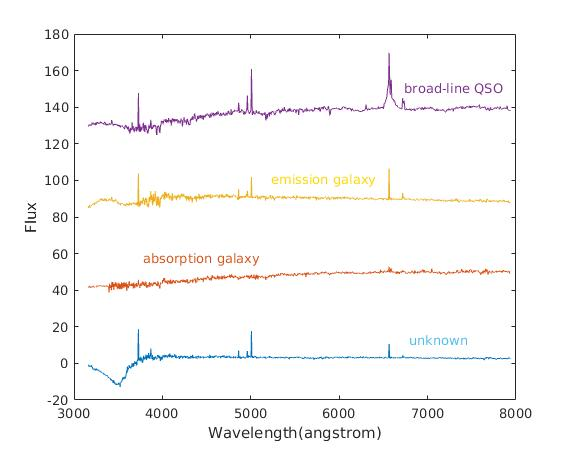
\includegraphics[scale=0.6]{sample_spec.jpg}
    \end{figure}
    
    We can observe the different characteristics of the spectra associated with each object:\newline
    Broad-line quasars have marked and large peak of emission in the emission, emission galaxies distinguish themself, from other type
    of galaxies, thanks to the presence of very narrow and high peak of emission(in general higher than narrow-line QSO); absorption 
    galaxies present a series of `caves` in their spectra where some component of the light is absorbed by particular chemical compounds present in 
    the objects of the galaxy; on the other hand `standard` galaxies present a spectra that rapresent a trdeoff between the previous cases.\newline\newline
    
    \noindent We also include a histogram showing the number of objects per class:
    \begin{figure}[H]
      \caption{Objects per class}
      \centering
      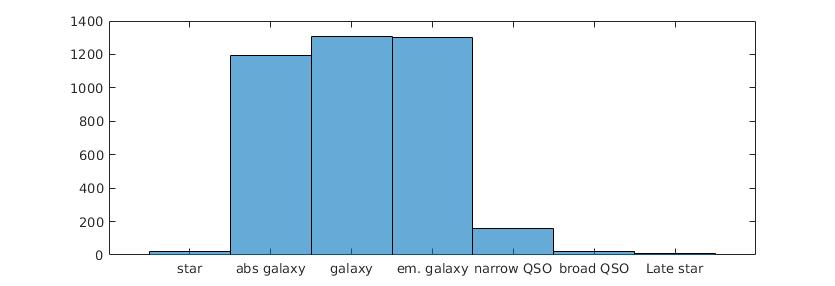
\includegraphics[scale=0.4]{histogram.jpg}
    \end{figure}
    The histogram shows a very irregular distribution of the objects in the class, this is due to two main reasons:
    \begin{enumerate}
     \item Some objects are more difficult to observe with respect to others, quasars are more rare to observe(and to discover) with respect to galaxies
     \item The dataset in consideration has a limited amount of samples(~4000), this is mainly due to the limited computational power available to the author. 
    \end{enumerate}

  
  \subsection{Metrics}
    The results of the different alternatives evaluated over the test set are compared according the confusion matrix.\newline
    The confusion matrix is $K x K$ matrix (in our case $K = 7$), the generic element $e_ij$ indicates how many samples 
    that comes from class $i$ have been predicted to class $j$.\newline
    The following metric can be evaluated:
    \begin{equation*}
     Accuracy = \frac{\sum_{i = 1}^K e_{ii}}{N} 
    \end{equation*}
    For each class $k$ we also consider:
    \begin{equation*}
     Precision_k = \frac{tp_k}{fp_k + tp_k} 
    \end{equation*}
    \begin{equation*}
     Recall_k = \frac{tp_k}{tp_k + fn_k} 
    \end{equation*}
    Where $tp_k$ is the number of true positive for class $k$, ie the number of samples that belong to class $k$ and has been
    correctly predicted to class $k$, and $fp_k$ is the number of false positive, ie the number of samples that does not belong
    to class $k$ but have been predicted to class $k$.\newline
    The precision express the number of correctly predicted samples for a given class $k$ with respect to the number of true positives plus
    the number of point that has been uncorrectly predicted belonging to class $k$.\newline
    The recall express the number of correctly predicted samples for a given class $k$ with respect to the number of true positives plus 
    the number of point that has been uncorrectly predicted not belonging to class $k$.
  \subsection{Results}
    \subsubsection{Baseline Classifier\protect\footnote{Refer to script baseline.m}}
      The first problem in SVM classification is the choice of the correct kernel:\newline
      Three different kernels have been evaluated, as a rough estimation of the performance we consider the classsification accuracy:
      \begin{itemize}
       \item Linear Kernel, Accuracy on the test set: $\sim$ 67\%
       \item Polynomial Kernel(3\textdegree \hspace{.1mm} polynom), Accuracy on the test set: $\sim$ 69\% 
       \item Gaussian Kernel, Accuracy on the test set: $\sim$ 33.5\%
      \end{itemize}
      The optimal hyper-parameter are chosen by 5-fold cross-validation.\newline
      This rough evaluation of these type of kernel shows how a gaussian kernel performs very bad over the test set mainly due to overfitting.\newline
      We decide to use a polynomial based kernel, follows a detailed analysis to find the best order for the polynom.\newline
      The generic polynomial kernel is in the form:
      \begin{equation}
       k(x,y) = (\gamma x^Ty)^d
      \end{equation}
      We perform a 5-fold cross-validation in order to determine the best $\gamma$, C and degree(d).\newline
      The procedure has individuated the following hyperparameter:
      \begin{itemize}
       \item degree(d) = 3
       \item $\gamma = 2^{-20} = 0,000000954$
       \item $C = 2^{15} = 32768$
      \end{itemize}
      \begin{figure}[H]
	\centering
	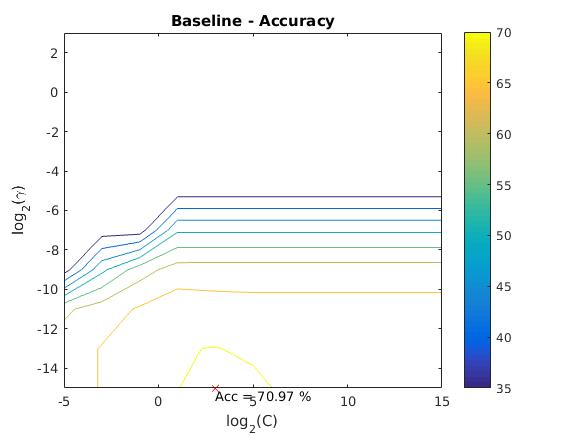
\includegraphics[scale=0.5]{baseline.jpg}
	\caption{Baseline Contour plot}
      \end{figure}
      With the optimal value of C and $\gamma$ the baseline classifier has been able to achieve on the test set an accuracy of 68.88 \% \newline
      \begin{figure}[H]
	\centering
	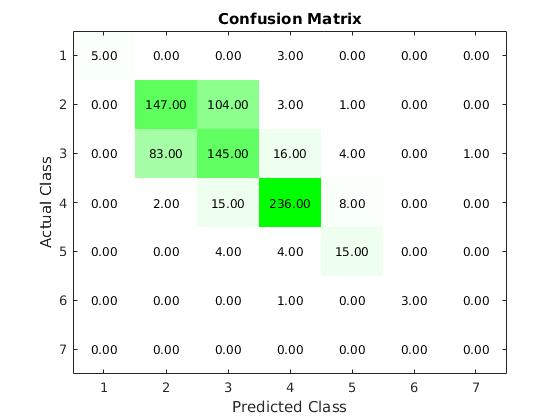
\includegraphics[scale=0.5]{conf_matrix_baseline.jpg}
	\caption{Baseline Heatmap}
      \end{figure}
      \noindent We also report the recall and precision for each class:\newline
      
      \begin{table}[H]
      	\centering
	\begin{tabular}{l|P{1cm}P{1cm}P{1cm}P{1cm}P{1cm}P{1cm}P{1cm}} \toprule
	  {$Class$} & {$1$} & {$2$} & {$3$} & {$4$} & {$5$} & {$6$} & {$7$} \\ \midrule
	  $Precision$  & 1 & 0.6336 & 0.5410 & 0.8973 & 0.5357 & 1 & 0 \\ \midrule
	  $Recall$  & 0.6250 & 0.5765 & 0.5823 & 0.9042 & 0.6522 & 0.75  & $NaN$  \\ \bottomrule
	\end{tabular}
      \end{table}
    
    \subsubsection{ANOVA Classifier\protect\footnote{Refer to script anova.py}}
      This section describes the first attempt to improve the performance of the baseline classifier by trying to reduce the number of
      features by calculating an univariate f-test over the features.\newline
      To have a rough idea on which may be the most informative features we plot the f-score(the results of the previous analysis) for each 
      feature: the higher the lower the p-value, a low p-value means a statistically significant feature.
      \begin{figure}[H]
	\centering
	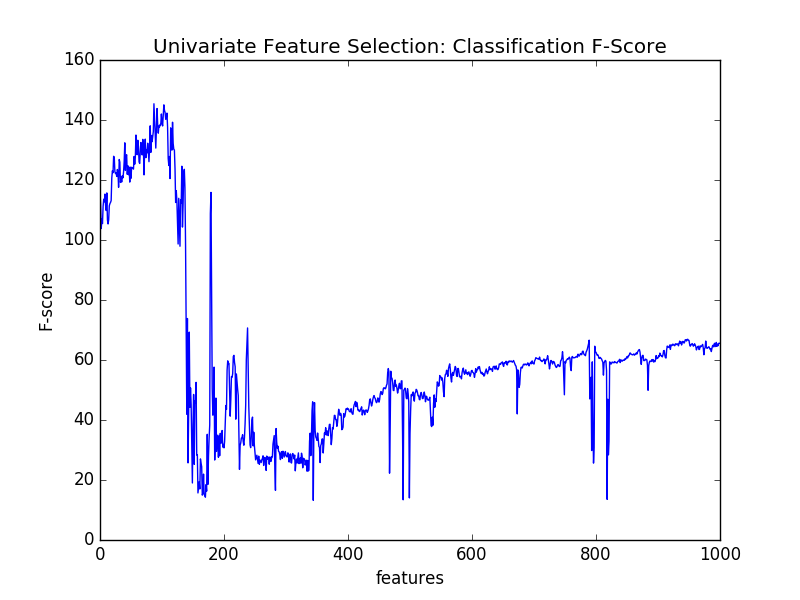
\includegraphics[scale=0.5]{anova_f_score.png}
	\caption{ANOVA F-Score}
      \end{figure}
      
      \noindent The graph clearly shows how the first 160 $\sim$ 180 features have a higher inoformative level with respect to the others.\newline
      We try different percentiles of features and using 5-fold cross validation we have calculated the accuracy; the results are shown in the following picture.
      \begin{figure}[H]
	\centering
	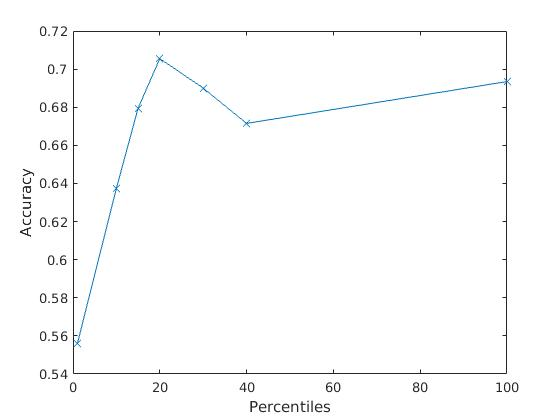
\includegraphics[scale=0.5]{anova-acc.jpg}
	\caption{ANOVA Accuracy-Percentile}
      \end{figure}
      \noindent The results clearly shows, as expected, how a smaller number of features($\sim$ 20\%) produce the maximum accuracy. \newline
      What follows is a more detaled analysis of the results over the test set.
      \begin{figure}[H]
	\centering
	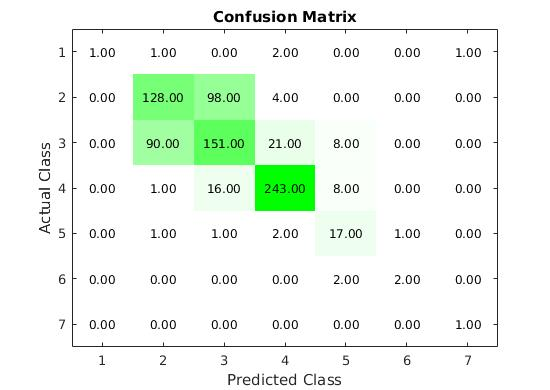
\includegraphics[scale=0.5]{anova-heat.jpg}
	\caption{ANOVA Heatmap}
      \end{figure}
      The table report precision and recall for each class.
      \begin{table}[H]
      	\centering
	\begin{tabular}{l|P{1cm}P{1cm}P{1cm}P{1cm}P{1cm}P{1cm}P{1cm}} \toprule
	  {$Class$} & {$1$} & {$2$} & {$3$} & {$4$} & {$5$} & {$6$} & {$7$} \\ \midrule
	  $Precision$  & 1 & 0.5792 & 0.5677 & 0.8934  & 0.4857 &  0.6667  & 0.5 \\ \midrule
	  $Recall$  & 0.2 &  0.5565 &  0.5593 & 0.9067 & 0.7727  & 0.5 & 1  \\ \bottomrule
	\end{tabular}
      \end{table}
      
     \subsubsection{PCA\protect\footnote{Refer to script pca.py}}
      This section describes the first attempt to improve the performance of the anova/baseline classifier by trying to use a more 
      sophisticated approach to the problem of dimensionality. 
      Features are not selected but the data are projected along their principal components.\newline
      The following picture shows the accuracy versus different number of selected components.
      \begin{figure}[H]
	\centering
	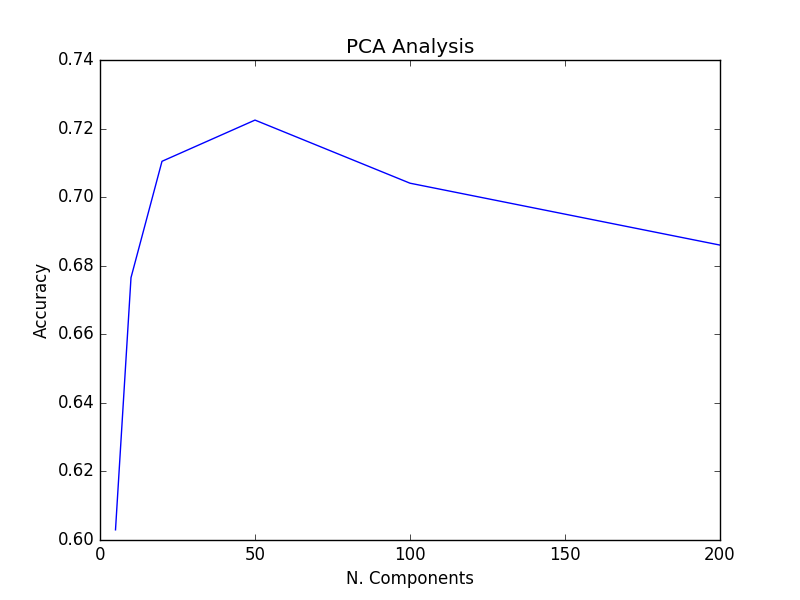
\includegraphics[scale=0.5]{pca-acc.png}
	\caption{PCA Accuracy-Components}
      \end{figure}
      \noindent The figure shows how a very small number of components($\sim$ 50) 
      can achieve an accuracy better than the baseline and ANOVA classifier.\newline
      What follows is a more detaled analysis of the results over the test set.
      \begin{figure}[H]
	\centering
	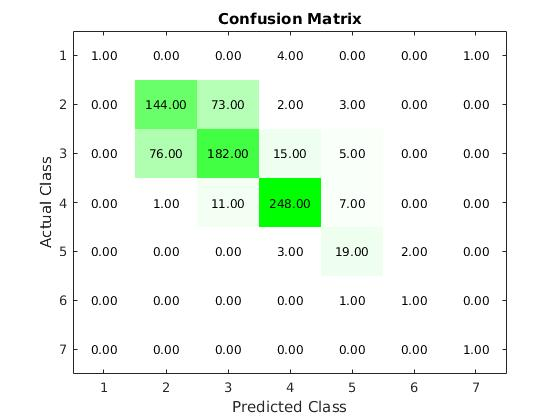
\includegraphics[scale=0.5]{pca-heat.jpg}
	\caption{PCA Heatmap}
      \end{figure}
      The table report precision and recall for each class.
      \begin{table}[H]
      	\centering
	\begin{tabular}{l|P{1cm}P{1cm}P{1cm}P{1cm}P{1cm}P{1cm}P{1cm}} \toprule
	  {$Class$} & {$1$} & {$2$} & {$3$} & {$4$} & {$5$} & {$6$} & {$7$} \\ \midrule
	  $Precision$  & 1  &  0.6516 & 0.6842 & 0.9118 & 0.5429 & 0.3333 & 0.5 \\ \midrule
	  $Recall$  & 0.1667 & 0.6486 & 0.6547 & 0.9288 & 0.7917 & 0.5000 & 1  \\ \bottomrule
	\end{tabular}
      \end{table}

     \subsubsection{Forward Features Selection\protect\footnote{Refer to script fwfs.py}}
      This section shows the results given by the approach described in section 3.3.
      The analysis stops when more than 200 features have been selected or when the algorithm reaches a local optima,
      ie. the difference between to subsequent scores is less than a given threshold(or tolerance in this case 0.001).\newline
      The execution of the relevant script selects the following features:\newline\newline
      \textbf{[963, 793, 759, 238, 867, 866, 875]}\newline\newline
      It is important to notice two important facts:
      \begin{itemize}
       \item The algorithm selects a very small number of features(7) in spite of the previuos techniques where the number of features 
	is higher
       \item The algorithm seems to prefer features located in the upper part of the spectrum while the previous ANOVA analysis 
	seem to prefer low frequency features
      \end{itemize}
      
      As usual we report the result over the test set:
      \begin{figure}[H]
	\centering
	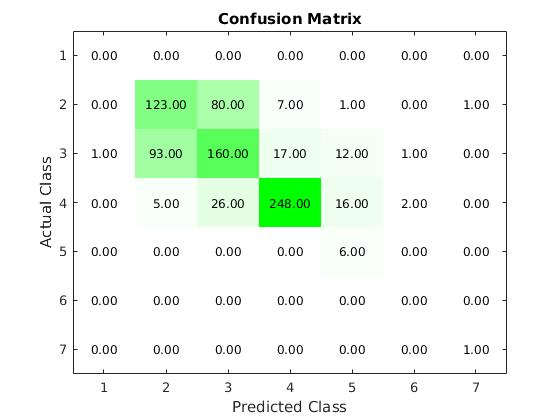
\includegraphics[scale=0.5]{fwfs-heat.jpg}
	\caption{FWFS Heatmap}
      \end{figure}
      The following table report precision and recall for each class.
      \begin{table}[H]
      	\centering
	\begin{tabular}{l|P{1cm}P{1cm}P{1cm}P{1cm}P{1cm}P{1cm}P{1cm}} \toprule
	  {$Class$} & {$1$} & {$2$} & {$3$} & {$4$} & {$5$} & {$6$} & {$7$} \\ \midrule
	  $Precision$  & 0 & 0.5566 & 0.6015 & 0.9118 & 0.1714 & 0 & 0.5 \\ \midrule
	  $Recall$  & $NaN$ & 0.5802 & 0.5634 & 0.8350 & 1 & $NaN$ & 1 \\ \bottomrule
	\end{tabular}
      \end{table}
     
     \subsubsection{ISOMAP\protect\footnote{Refer to script isomap.py}}
      This section describes a second attempt to improve the performance of the PCA classifier by trying to use a more 
      sophisticated approach to the problem of dimensionality. 
      Isomap exploits geodesic paths for nonlinear dimensionality reduction.\newline
      The following picture shows the accuracy versus different number of selected components and neighbors.
      \begin{figure}[H]
	\centering
	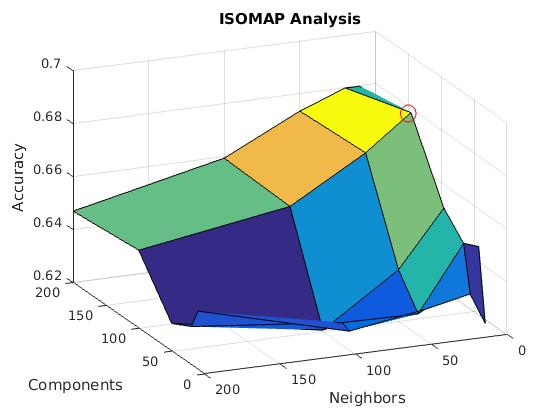
\includegraphics[scale=0.5]{iso-acc.jpg}
	\caption{ISOMAP Accuracy-Components-Neighbors}
      \end{figure}
      \noindent The figure shows how a very small number of components($\sim$ 50) 
      can achieve an accuracy better than the baseline and ANOVA classifier.\newline
      What follows is a more detaled analysis of the results over the test set.
      \begin{figure}[H]
	\centering
	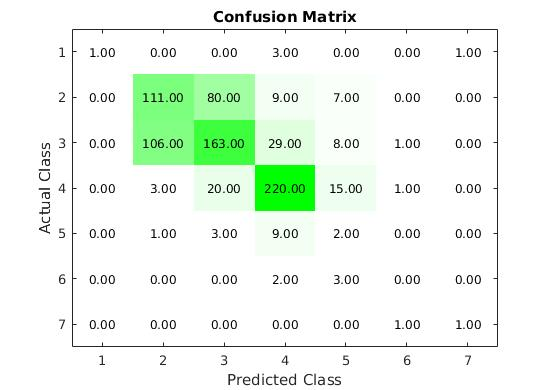
\includegraphics[scale=0.5]{iso-heat.jpg}
	\caption{ISOMAP Heatmap}
      \end{figure}
      The following table report precision and recall for each class.
      \begin{table}[H]
      	\centering
	\begin{tabular}{l|P{1cm}P{1cm}P{1cm}P{1cm}P{1cm}P{1cm}P{1cm}} \toprule
	  {$Class$} & {$1$} & {$2$} & {$3$} & {$4$} & {$5$} & {$6$} & {$7$} \\ \midrule
	  $Precision$  & 1 & 0.5023 & 0.6128 & 0.8088 & 0.0571 & 0 & 0.5 \\ \midrule
	  $Recall$  & 0.2 & 0.5362 & 0.5309 & 0.8494 & 0.1333 & 0 & 0.5 \\ \bottomrule
	\end{tabular}
      \end{table}
      \noindent It is important to point out how the SVM trained after performing the ISOMAP reduction perform worse on the 
      the test set(accuracy: $\sim$63\%) with respect to the PCA classifier.\newline
      It is quite complicated understand the reasons behind the this performance degradation, we suppose this is mainly due to 
      the lack of samples used during the analysis indeed others works \cite{sdssiso} outlined that with a much higher number of
      data ISOMAP outperform PCA.
    
\newpage

\section{Conclusions}

\newpage

\begin{thebibliography}{9}
  \bibitem{spectrum}
    Wikipedia,
    \emph{Emission Spectrum}
    
   \bibitem{sdss}
    Wikipedia,
    \emph{The Sloan Digital Sky Survey}
    
   \bibitem{redshift}
    C.W. Yip et al,
    \emph{Spectral Classification of Quasars in the Sloan Digital Sky Survey: Eigenspectra, Redshift, and Luminosity Effects},
    Astronomical Journal,
    2004
    
   \bibitem{multisvm}
    Chih-Wei Hsu, Chih-Jen Lin,
    \emph{A Comparison of Methods for Multi-class Support Vector Machines},
    IEEE Transactions on Neural Networks, 13(2002), 415-425
    
   \bibitem{libsvm}
    Chih-Wei Hsu, Chih-Jen Lin,
    \emph{LibSVM: A Library for Support Vector Machines},
    https://www.csie.ntu.edu.tw/~cjlin/libsvm/
    
   \bibitem{openmpsvm}
    Chih-Wei Hsu, Chih-Jen Lin,
    \emph{Use OpenMP to parallelize LibSVM on a multicore/shared-memory computer},
    http://www.csie.ntu.edu.tw/~cjlin/libsvm/faq.html\#f432
    
   \bibitem{sdssiso}
    Bu Yude, Chen Fuqiang, Pan Jingchang,
    \emph{Stellar spectral subclasses classification based on Isomap and SVM},
    New Astronomy, Volume 28, p. 35-43.
    
\end{thebibliography}

\end{document}
